\documentclass[preview]{standalone}

\usepackage{amsmath}
\usepackage{amssymb}
\usepackage{bettelini}
\usepackage{stellar}
\usepackage{definitions}
\usepackage{wrapfig}

\begin{document}

\id{measuretheory-fubini-tonelli}
\genpage

\section{Tonelli's Theorem}

\begin{snippettheorem}{tonelli-theorem}{Tonelli's theorem}
    Let \((X,\mathcal M,\mu)\) and \((Y,\mathcal S,\lambda)\) be
    \(\sigma\)-finite measure spaces, and let
    \(f\colon X\cartesianprod Y\fromto[0,+\infty]\) be
    \((\mathcal M\cartesianprod\mathcal S)\)-measurable. Then
    \[
        x\longmapsto\int_Yf(x,y)\,d\lambda(y),
        \qquad
        y\longmapsto\int_Xf(x,y)\,d\mu(x)
    \]
    are measurable, possibly extended-valued functions, and
    \[
        \int_{X\cartesianprod Y}f\,d(\mu\times\lambda)
        =
        \int_X\left(\int_Yf(x,y)\,d\lambda(y)\right)d\mu(x)
        =
        \int_Y\left(\int_Xf(x,y)\,d\mu(x)\right)d\lambda(y).
    \]
\end{snippettheorem}

\section{Fubini's Theorem}

\begin{snippettheorem}{fubini-theorem}{Fubini's theorem}
    Let \((X,\mathcal M,\mu)\) and \((Y,\mathcal S,\lambda)\) be
    \(\sigma\)-finite measure spaces, and let
    \(f\in\mathcal L^1(\mu\times\lambda)\). Then:
    \begin{enumerate}
        \item \(f_x(y)=f(x,y)\) belongs to \(\mathcal L^1(\lambda)\) for
            almost every \(x\), and
            \(f^y(x)=f(x,y)\) belongs to \(\mathcal L^1(\mu)\) for almost
            every \(y\);
        \item the functions
            \[
                x\longmapsto\int_Yf_x\,d\lambda,
                \qquad
                y\longmapsto\int_Xf^y\,d\mu
            \]
            are integrable after arbitrary definitions on their exceptional
            null sets;
        \item
            \[
                \int_{X\cartesianprod Y}f\,d(\mu\times\lambda)
                =
                \int_X\left(\int_Yf_x\,d\lambda\right)d\mu
                =
                \int_Y\left(\int_Xf^y\,d\mu\right)d\lambda.
            \]
    \end{enumerate}
\end{snippettheorem}

\begin{snippet}{tonelli-fubini-distinction}
    Tonelli's theorem assumes nonnegativity and permits the value
    \(+\infty\). Fubini's theorem allows real or complex functions of
    arbitrary sign, but requires integrability on the product space. The
    sections in Fubini's theorem may fail to be integrable on exceptional
    null sets.
\end{snippet}

\begin{snippettheorem}{tonelli-integrability-criterion}{Tonelli's integrability criterion}
    Under the same \(\sigma\)-finiteness assumptions, let
    \(f\colon X\cartesianprod Y\fromto\complexnumbers\) be
    \((\mathcal M\cartesianprod\mathcal S)\)-measurable. If either iterated
    integral
    \[
        \int_X\left(\int_Y|f(x,y)|\,d\lambda(y)\right)d\mu(x)
    \]
    or the analogous expression in the reverse order is finite, then
    \(f\in\mathcal L^1(\mu\times\lambda)\). Consequently, Fubini's theorem
    applies in both orders.
\end{snippettheorem}

\begin{snippet}{iterated-integrals-do-not-characterize-integrability}
    Merely computing both iterated integrals of \(f\), even if they exist and
    agree, does not prove that \(f\in\mathcal L^1(\mu\times\lambda)\). One
    must instead establish measurability and absolute integrability, for
    example through Tonelli's criterion.
\end{snippet}

\section{Counterexamples}

\begin{snippetexample}{equal-iterated-integrals-nonintegrable-function}{Equal iterated integrals without product integrability}
    \begin{wrapfigure}{r}{6cm}
        \begin{center}
            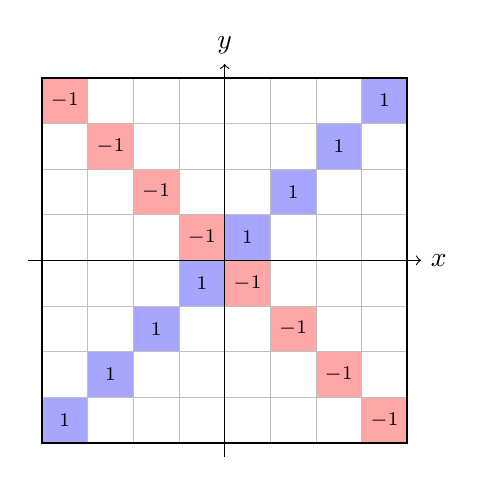
\begin{tikzpicture}[x=0.58cm,y=0.58cm]
                \foreach \n in {-4,-3,...,3}{
                    \fill[blue!35] (\n,\n) rectangle ++(1,1);
                    \fill[red!35] (\n,{-\n-1}) rectangle ++(1,1);
                }
                \draw[step=1,gray!50,very thin] (-4,-4) grid (4,4);
                \draw[thick] (-4,-4) rectangle (4,4);
                \draw[->] (-4.3,0) -- (4.3,0) node[right] {$x$};
                \draw[->] (0,-4.3) -- (0,4.3) node[above] {$y$};
                \foreach \n in {-4,-3,...,3}{
                    \node at ({\n+0.5},{\n+0.5}) {\scriptsize $1$};
                    \node at ({\n+0.5},{-\n-0.5}) {\scriptsize $-1$};
                }
            \end{tikzpicture}
            \vspace{-1cm}
        \end{center}
    \end{wrapfigure}
    Let \(X=Y=\realnumbers\) with Lebesgue measure. Define \(f=1\) on the
    unit squares meeting the diagonal, \(f=-1\) on those meeting the other
    diagonal, and \(f=0\) elsewhere. Every vertical section contains one
    positive and one negative unit interval, so its integral is zero. The
    same holds for every horizontal section. Both iterated integrals are
    therefore zero, but
    \[
        \int_{\realnumbers^2}|f|\,d\mu_2=+\infty.
    \]
    Thus \(f\notin\mathcal L^1(\realnumbers^2)\).
    \wrapfill
\end{snippetexample}

\begin{snippetexample}{different-iterated-integrals-nonintegrable-function}{Iterated integrals with different values}
    \begin{wrapfigure}{r}{6cm}
        \begin{center}
            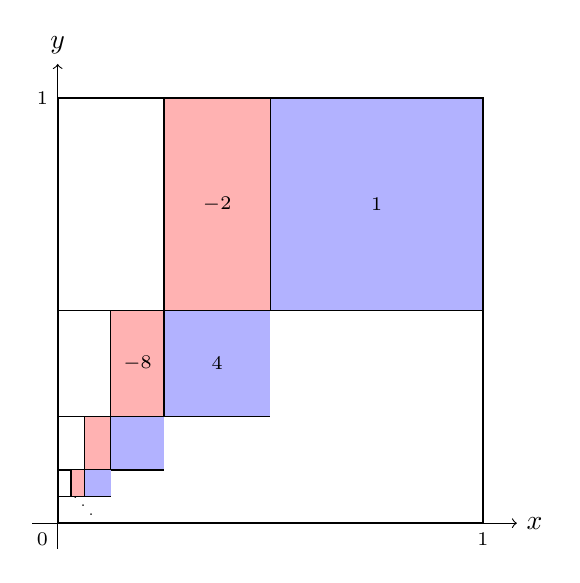
\begin{tikzpicture}[x=5.4cm,y=5.4cm]
                \foreach \n in {0,1,2,3}{
                    \pgfmathsetmacro{\a}{pow(2,-\n)}
                    \pgfmathsetmacro{\b}{pow(2,-\n-1)}
                    \pgfmathsetmacro{\c}{pow(2,-\n-2)}
                    \fill[blue!30] (\b,\b) rectangle (\a,\a);
                    \fill[red!30] (\c,\b) rectangle (\b,\a);
                    \draw[thin] (0,\b) -- (\a,\b);
                    \draw[thin] (\b,\b) -- (\b,\a);
                    \draw[thin] (\c,\b) -- (\c,\a);
                }
                \node at (0.75,0.75) {\scriptsize $1$};
                \node at (0.375,0.75) {\scriptsize $-2$};
                \node at (0.375,0.375) {\scriptsize $4$};
                \node at (0.1875,0.375) {\scriptsize $-8$};
                \node at (0.06,0.06) {\tiny $\ddots$};
                \draw[thick] (0,0) rectangle (1,1);
                \draw[->] (-0.06,0) -- (1.08,0) node[right] {$x$};
                \draw[->] (0,-0.06) -- (0,1.08) node[above] {$y$};
                \node[below left] at (0,0) {\scriptsize $0$};
                \node[below] at (1,0) {\scriptsize $1$};
                \node[left] at (0,1) {\scriptsize $1$};
            \end{tikzpicture}
            \vspace{-1.25cm}
        \end{center}
    \end{wrapfigure}
    Extend the pattern displayed in the figure indefinitely toward the
    origin. Every horizontal section integrates to zero. In the other order,
    all contributions cancel except on \(x\in[1/2,1]\), where the vertical
    integral equals \(1/2\). Hence
    \[
        \int_\realnumbers\left(\int_\realnumbers f(x,y)\,dx\right)dy=0,
    \]
    whereas
    \[
        \int_\realnumbers\left(\int_\realnumbers f(x,y)\,dy\right)dx
        =\int_{1/2}^{1}\frac12\,dx=\frac14.
    \]
    The function is not in \(\mathcal L^1(\mu_2)\), since integrating its
    absolute value produces a divergent series.
    \wrapfill
\end{snippetexample}

\end{document}
